% Generated by `python -m experiments.experiment_4.appendix_captions` -- do not edit by hand.
% Appendix figures for Experiment 4. Needs \usepackage{graphicx,subcaption}; paths are relative to outputs/finals/experiment-4/.

\begin{figure}[p]
  \centering
  \begin{subfigure}{\textwidth}\centering
    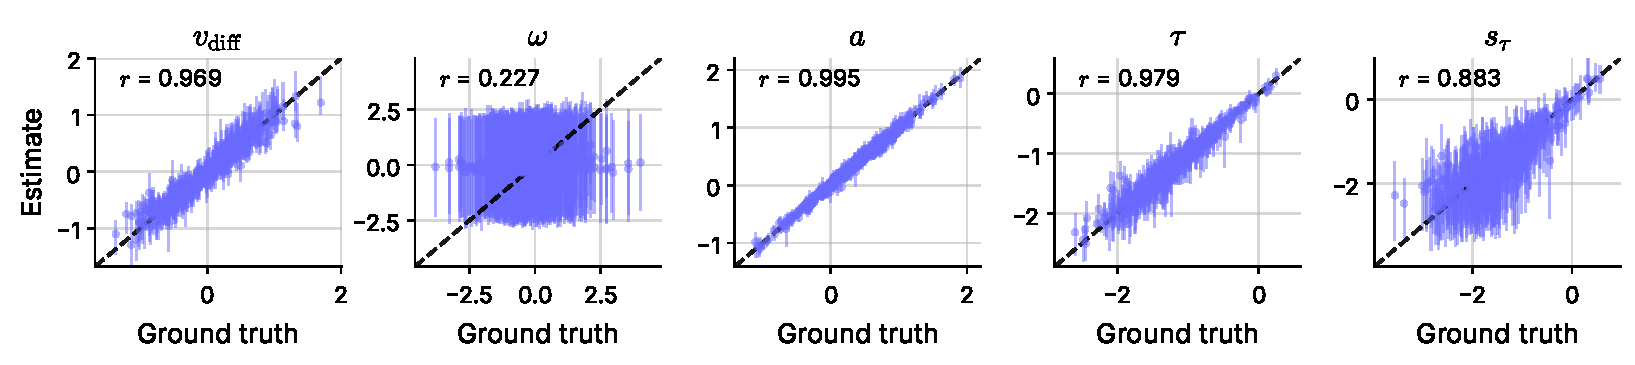
\includegraphics[width=\textwidth]{probe/baseline/recovery.pdf}
    \caption{Recovery}
  \end{subfigure}\\[1ex]
  \begin{subfigure}{\textwidth}\centering
    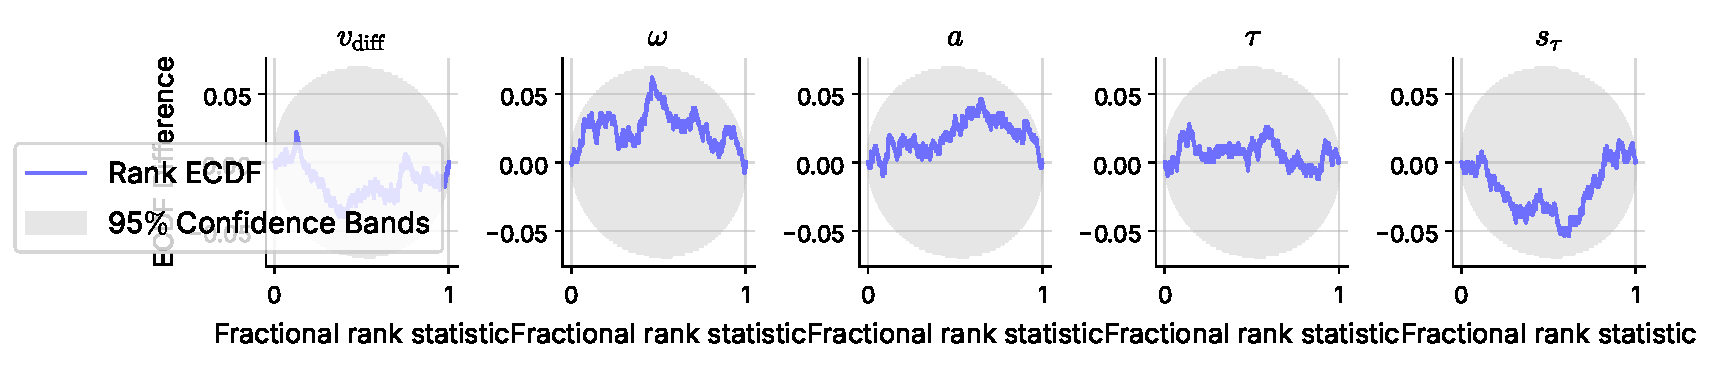
\includegraphics[width=\textwidth]{probe/baseline/calibration_ecdf.pdf}
    \caption{Calibration (ECDF)}
  \end{subfigure}\\[1ex]
  \begin{subfigure}{\textwidth}\centering
    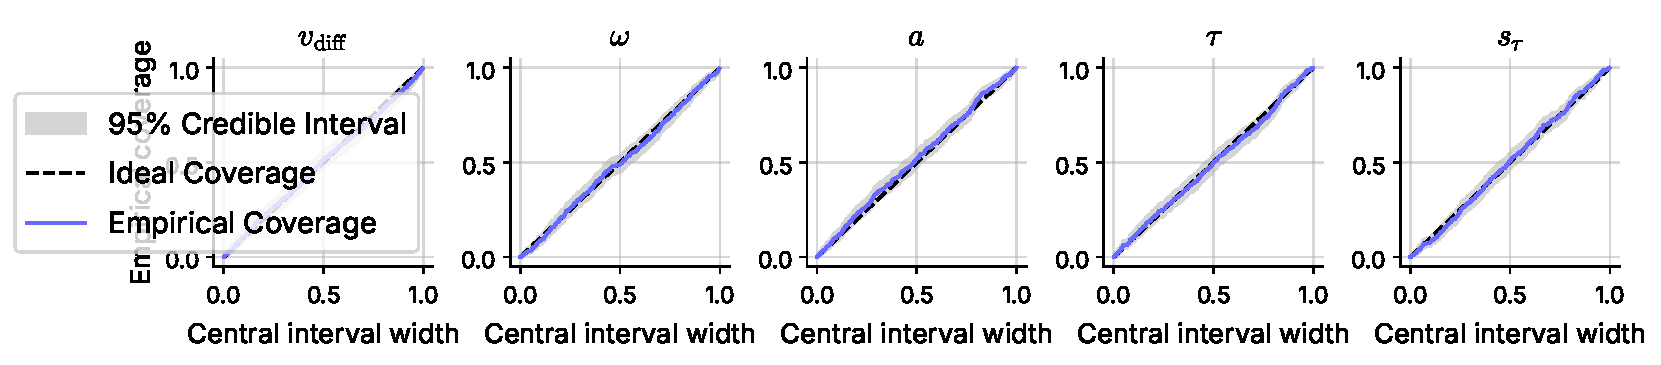
\includegraphics[width=\textwidth]{probe/baseline/coverage.pdf}
    \caption{Coverage}
  \end{subfigure}\\[1ex]
  \begin{subfigure}{\textwidth}\centering
    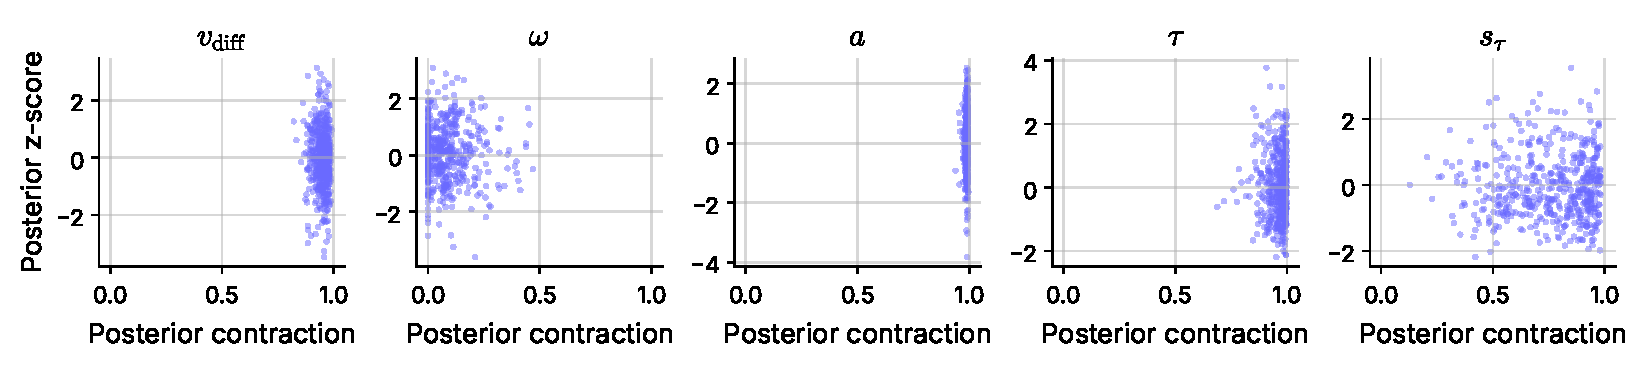
\includegraphics[width=\textwidth]{probe/baseline/z_score_contraction.pdf}
    \caption{$z$-score vs contraction}
  \end{subfigure}
  \caption{\textbf{aDDM, learned SetTransformer summary (baseline arm): diagnostics.} (a) Recovery: posterior medians against ground truth with central 95\% credible intervals, $r$ their correlation; (b) calibration: rank-ECDF difference (empirical minus uniform) with simultaneous 95\% bands; (c) coverage: empirical against nominal coverage of central credible intervals; (d) posterior $z$-score against posterior contraction, one point per dataset. 500 validation datasets of 500 trials with 500 posterior draws each, on the unconstrained scale. Contraction (NRMSE) per parameter: $v_{\mathrm{diff}}$ 0.95 (0.22), $\omega$ 0.07 (0.96), $a$ 0.99 (0.10), $\tau$ 0.98 (0.17), $s_\tau$ 0.80 (0.46). $\omega$'s posterior stays close to its prior, so its calibration is almost automatic; the informative tests are the contracted parameters. Figure~\ref{fig:app4-arm-frozen} has the same layout for the frozen arm.}
  \label{fig:app4-arm-baseline}
\end{figure}

\begin{figure}[p]
  \centering
  \begin{subfigure}{\textwidth}\centering
    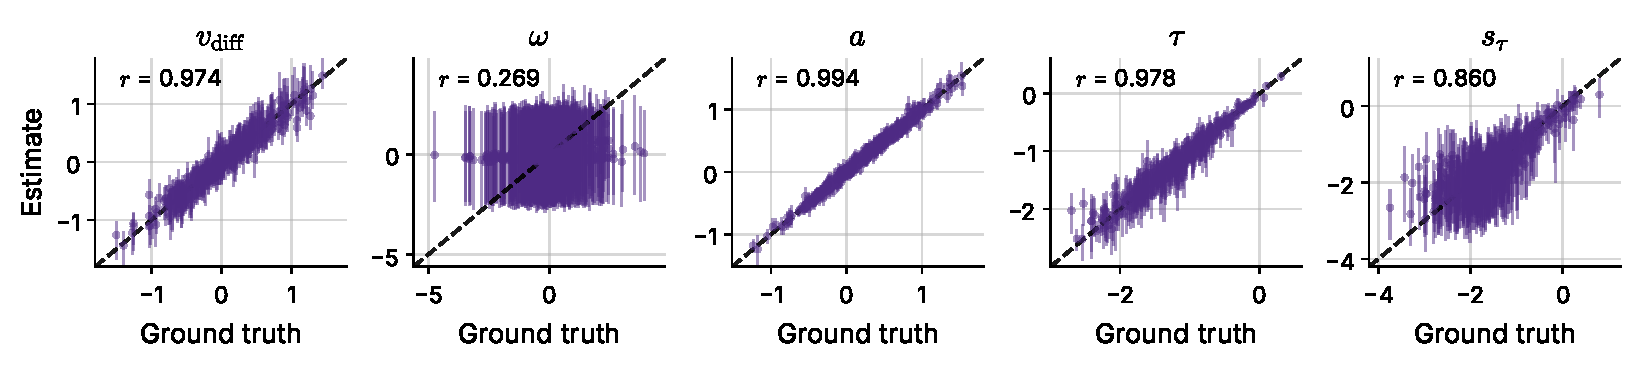
\includegraphics[width=\textwidth]{probe/frozen/recovery.pdf}
    \caption{Recovery}
  \end{subfigure}\\[1ex]
  \begin{subfigure}{\textwidth}\centering
    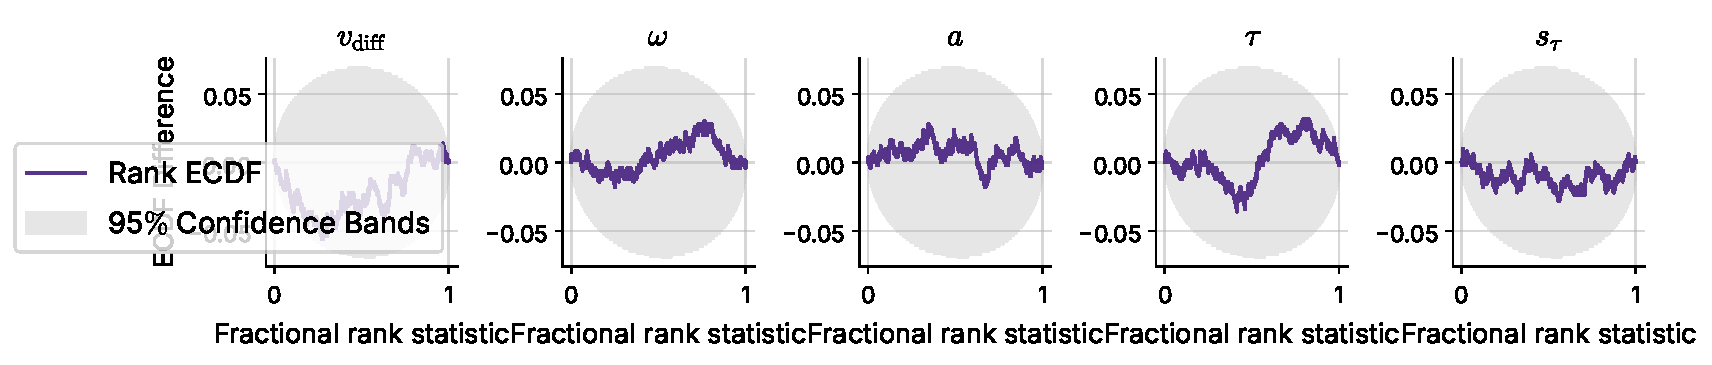
\includegraphics[width=\textwidth]{probe/frozen/calibration_ecdf.pdf}
    \caption{Calibration (ECDF)}
  \end{subfigure}\\[1ex]
  \begin{subfigure}{\textwidth}\centering
    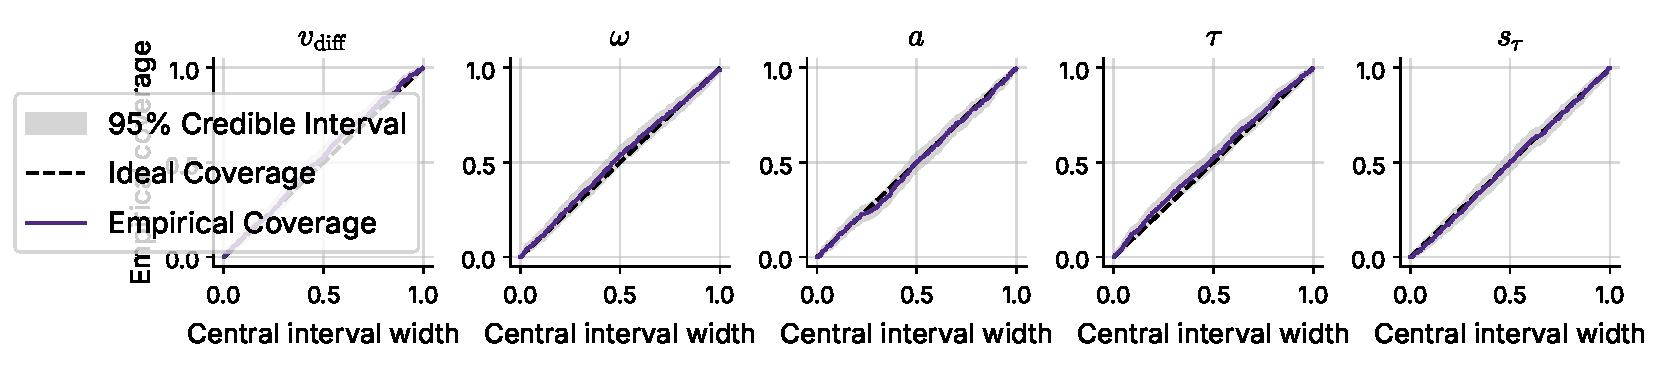
\includegraphics[width=\textwidth]{probe/frozen/coverage.pdf}
    \caption{Coverage}
  \end{subfigure}\\[1ex]
  \begin{subfigure}{\textwidth}\centering
    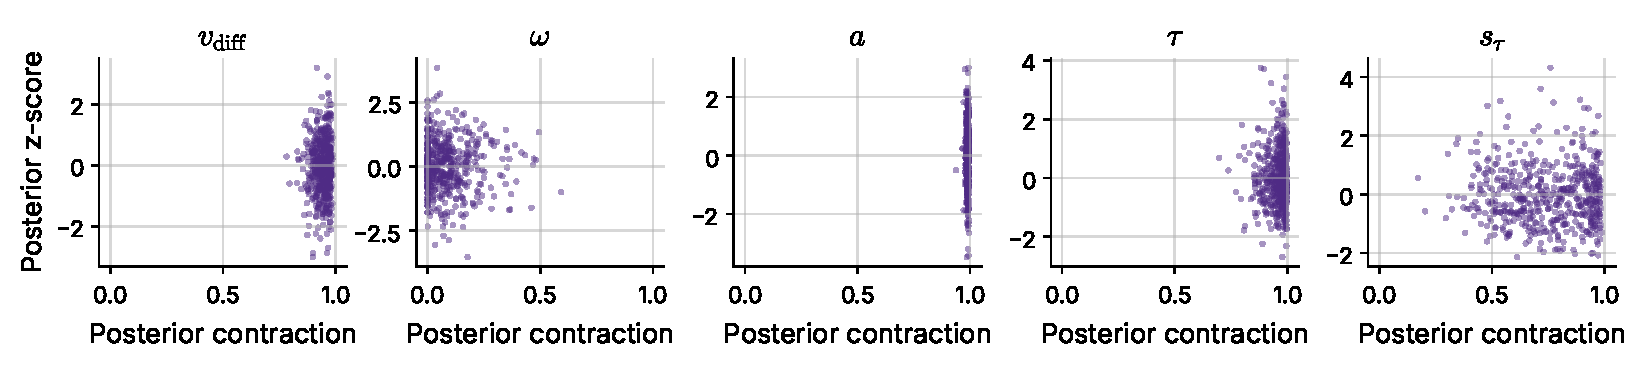
\includegraphics[width=\textwidth]{probe/frozen/z_score_contraction.pdf}
    \caption{$z$-score vs contraction}
  \end{subfigure}
  \caption{\textbf{aDDM, frozen CogFormer encoder (frozen arm): diagnostics.} (a) Recovery, (b) calibration, (c) coverage, (d) $z$-score against contraction, as in Figure~\ref{fig:app4-arm-baseline}. Contraction (NRMSE): $v_{\mathrm{diff}}$ 0.95 (0.24), $\omega$ 0.06 (0.96), $a$ 0.99 (0.11), $\tau$ 0.97 (0.18), $s_\tau$ 0.76 (0.52). Each arm is validated on its own simulated datasets, so the two figures are not paired; Figure~\ref{fig:app4-compare} compares the arms on shared data.}
  \label{fig:app4-arm-frozen}
\end{figure}

\begin{figure}[p]
  \centering
  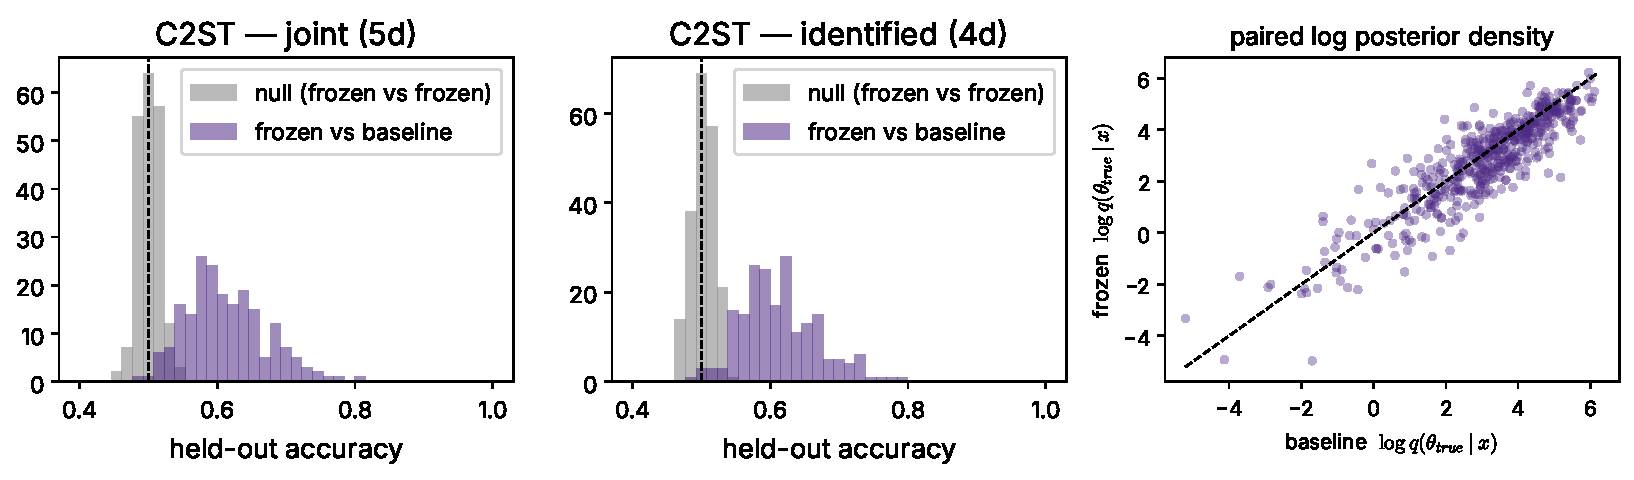
\includegraphics[width=\textwidth]{probe/compare/comparison.pdf}
  \caption{\textbf{aDDM: the two arms on shared data.} Both trained posteriors are applied to one set of 500 simulated datasets (500 trials), with 500 draws per arm. (a, b) Per-dataset classifier two-sample test (C2ST) on 200 of these datasets: held-out accuracy of a classifier (MLP, 5-fold cross-validation) trained to tell the frozen arm's draws from the baseline's (purple), against an empirical null from two independent sampling calls of the frozen arm (grey), which carries the same finite-sample bias; 0.5 (dashed) means indistinguishable. (a) Jointly over all 5 parameters: mean 0.612 against 0.501, excess $+0.111 \pm 0.004$ ($z = 26.0$). (b) Over the 4 identified parameters (contraction at least 0.5 in both arms; $\omega$ excluded), where agreement cannot be inherited from a shared prior: 0.613 against 0.502, excess $+0.111 \pm 0.004$ ($z = 27.1$). (c) Log posterior density of the true parameters, frozen against baseline, paired over the 500 datasets (dashed: equality): mean 2.77 against 3.04, paired difference $-0.27 \pm 0.04$ ($z = -7.1$; frozen higher on 36\% of datasets). C2ST is computed per dataset because pooled over datasets, two calibrated posteriors both average to the prior and the test reads 0.5 whatever their differences.}
  \label{fig:app4-compare}
\end{figure}

\begin{figure}[p]
  \centering
  \begin{subfigure}{\textwidth}\centering
    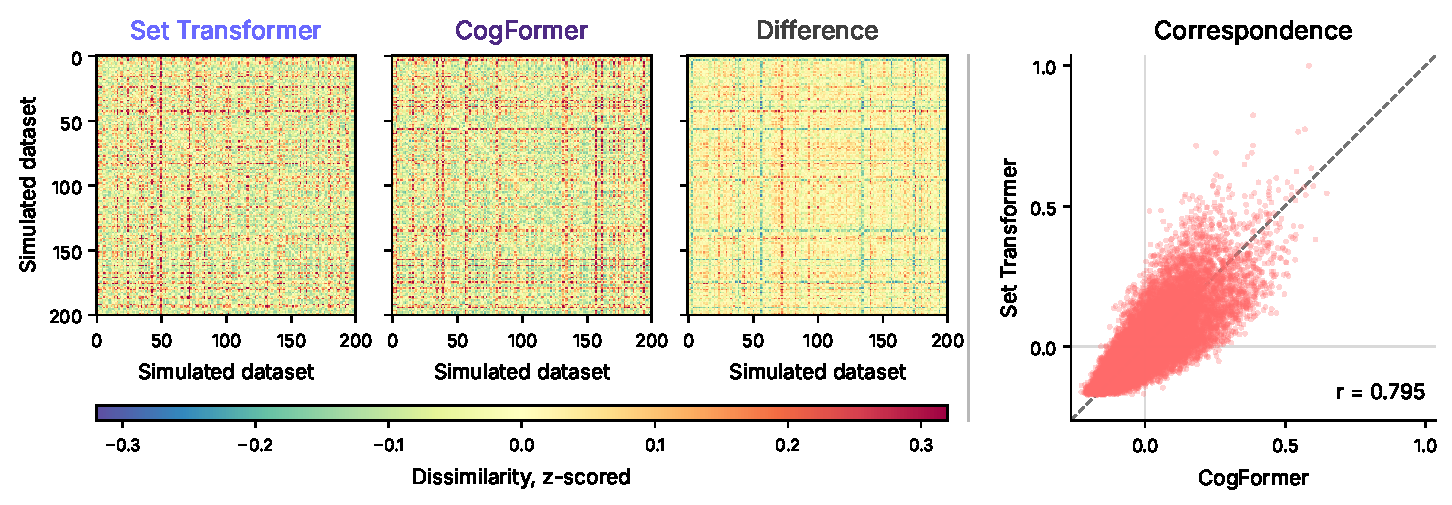
\includegraphics[width=\textwidth]{representation/frozen_vs_learned/rdm_rsa.pdf}
    \caption{}
  \end{subfigure}\\[1ex]
  \begin{subfigure}{0.48\textwidth}\centering
    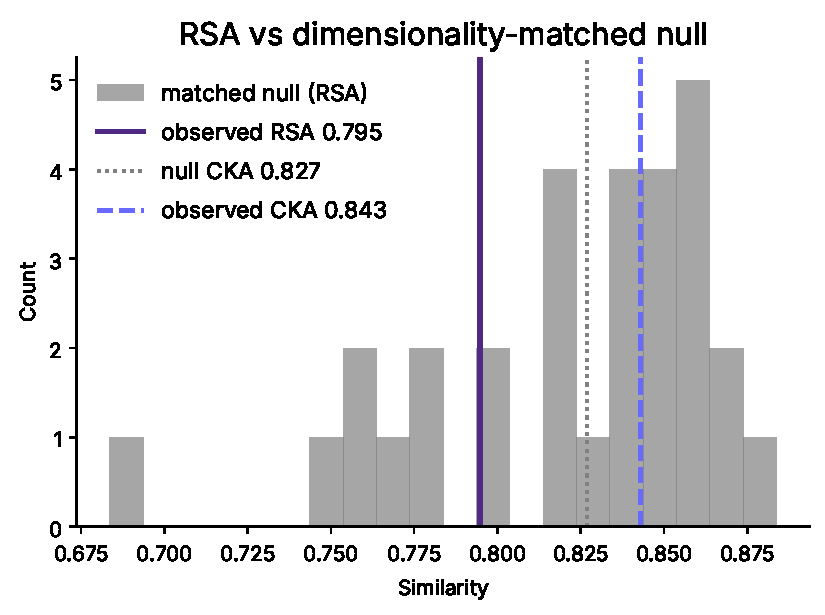
\includegraphics[width=\textwidth]{representation/frozen_vs_learned/rsa_vs_null.pdf}
    \caption{}
  \end{subfigure}\hfill
  \begin{subfigure}{0.48\textwidth}\centering
    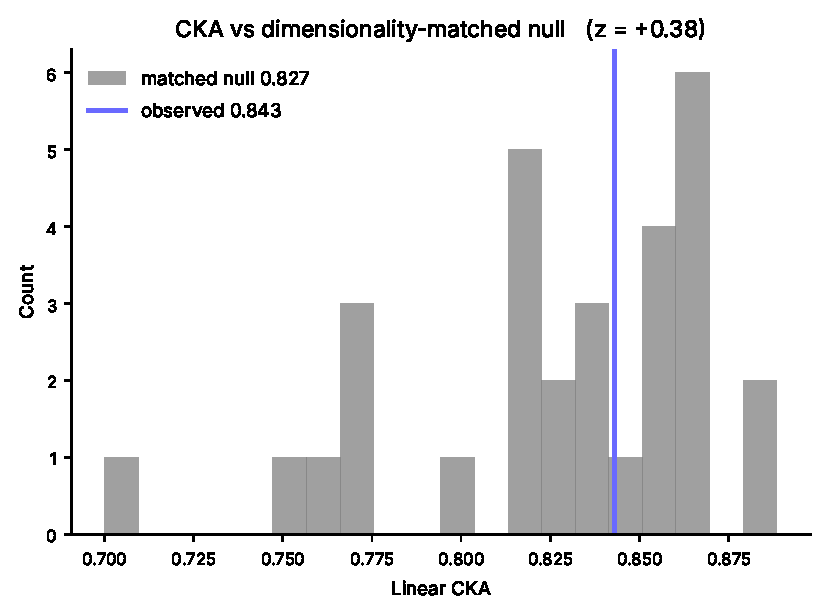
\includegraphics[width=\textwidth]{representation/frozen_vs_learned/cka_vs_null.pdf}
    \caption{}
  \end{subfigure}
  \caption{\textbf{aDDM: representational similarity of the two summaries.} (a) Representational dissimilarity matrices over 200 aDDM parameter draws, each simulated 4 times independently (500 trials): the learned SetTransformer summary (16 dimensions), the frozen CogFormer encoder (128), their difference (SetTransformer minus CogFormer), and their off-diagonal entries against each other. Dissimilarities are crossnobis distances, cross-validated over the 4 repeats so that measurement noise does not inflate them. The two summaries' distances are on different scales, so each matrix is z-scored over its off-diagonal entries (the normalisation Pearson correlation applies) and both are divided by one common constant; values are therefore signed and read as more or less dissimilar than typical, not as distances from zero. $r = 0.795$ is the Pearson correlation of the two off-diagonal vectors. (b) The observed RSA against the reference labelled ``matched null'': the frozen RDM compared with the RDMs of 30 random linear projections of the frozen summary itself to 16 dimensions ($0.821 \pm 0.044$). These projections keep the frozen encoder's own geometry up to compression loss, so the reference marks what a 16-dimensional linear readout of the frozen representation scores, not the absence of shared structure. Observed and reference CKA are marked for comparison. (c) The same for linear CKA: observed 0.843 against $0.827 \pm 0.043$ ($z = +0.38$). The CKA Gram block is in Figure~\ref{fig:exp4-main} (bottom right).}
  \label{fig:app4-rsa}
\end{figure}
